% ---------------------------- comment out when compiling the full document -------------------
\documentclass[twoside,11pt]{article}  % default square logo 
\usepackage{amssymb}
\usepackage{caption}
\usepackage{upgreek}
\usepackage{subfig}
\usepackage{textcomp}
\usepackage{graphicx}


\begin{document}
\baselineskip=15pt
% ---------------------------------------------------------------------------------------------------------------

\begin{figure}[!t]
\centering
\includegraphics[width=0.8\textwidth]{D0-add} \label{}
\caption{Radial distance of the projected tracks from the interaction point as recorded by a DBM telescope. The red, blue, yellow and green lines mark the inner and the outer radius of the beam pipe, the outer radius of the IBL and the outer radius of the IBL insertion tube.}
\end{figure}

\begin{figure}[!t]
\centering
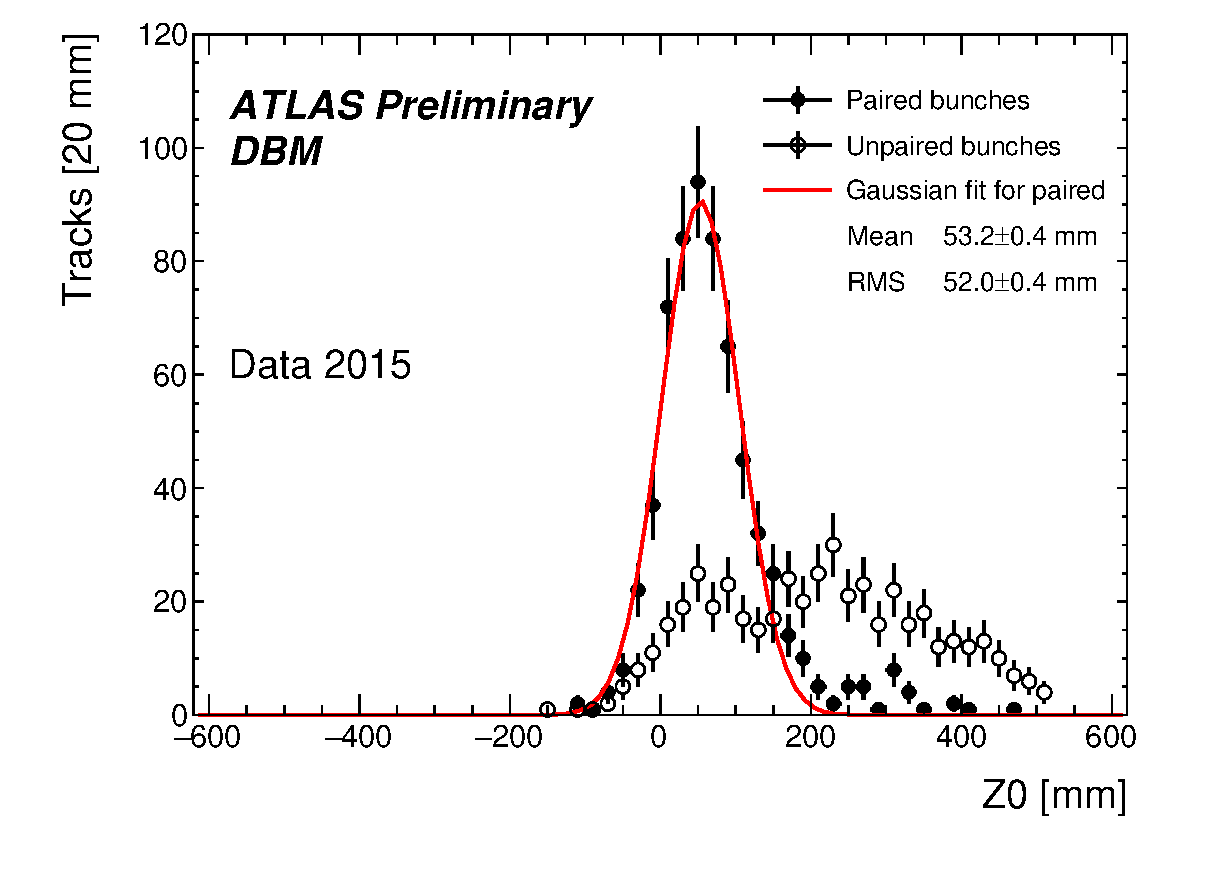
\includegraphics[width=0.8\textwidth]{Z0} \label{}
\caption{Longitudinal distance of the projected particle tracks from the interaction point as recorded by a DBM telescope.}
\end{figure}

% ---------------------------- comment out when compiling the full document -------------------
\end{document}
% ---------------------------------------------------------------------------------------------------------------
